\section{Protocolli di Trasporto}
I protocolli di trasporto sono un insieme di protocolli che risiedono sugli host e sugli endsystems; si occupano di fornire le regole per una comunicazione logica tra due entità remote.\\
A livello di invio, si occupano della ricezione dei messaggi in segmenti e li inviano al network layer; alla ricezione, i segmenti sono riassemblati in messaggi e passati al livello applicativo.\\
Mentre il livello di rete offre comunicazione tra due endsystems (trasportando informazioni da un host all'altro), il livello di trasporto crea un collegamento logico tra due \textit{processi}. Deve quindi essere in grado di raccogliere flussi informativi, utilizzare il livello di rete per trasportarli e successivamente smistarli nei vari processi applicativi.

\section{Internet transport-layer protocols}
A dispetto del fatto che il livello rete utilizza una best-effort policy che non dà nessuna garanzia di consegna, \textbf{TCP} si occuperà di applicare meccanismi per la traduzione di informazioni agli opportuni processi anche nel caso di perdita di dati.\\
I principali tipi di perdita dei dati sono:
\begin{itemize}
	\item un eccesso di informazioni arrivate al router intermedio. \\
	La conseguenza è un riempimento delle code fino al raggiungimento di una congestione in rete e all'inizio di una perdita di pacchetti.
	\item il ricevimento a destinazione di un tasso di informazioni troppo elevato rispetto alla velocità di lettura. \\
\end{itemize}
Si noti che un controllo del flusso di informazioni richiede algoritmi diversi rispetto al controllo di congestione; entrambi i tipi di controllo sono implementati da TCP.

\section{Multiplexing e Demultiplexing}
L'invio di informazioni da parte di un processo è eseguito attraverso una determinata porta dotata di interfacce ben definite. Tale porta, che consente il colloqui con l'entità sottostante di livello trasporto, prende il nome di \textit{socket}.\\
Poiché più flussi informativi sono trasmessi tramite lo stesso canale logico, occorre stabilire delle funzioni di smistamento di dati. Queste funzioni sono implementate nei protocolli TCP e UDP in maniera differente.\\

\subsection{UDP: Connectionless demux}
Il socket creato è dotato di un numero di porta dell'host locale; quando viene creato un \textit{datagram} (pacchetto) da inviare nel socket UDP, questo deve specificare l'indirizzo IP e il numero di porta dell'host di destinazione.
Quando l'host remoto riceve un segmento via UDP, controlla il suo numero di porta di destinazione e lo indirizza alla porta corrispondente.
Pacchetti con stesso numero di porta di destinazione, ma indirizzi IP o porte di origine differenti saranno quindi orientati allo stesso socket a destinazione.

\section{TCP: Connection-oriented demux}
In questo caso viene creato un socket dedicato al flusso di informazioni identificato dalla presenza di quattro campi: due per gli indirizzi IP del mittente e del destinatario, due per i numeri di porta del mittente e del destinatario.
Nel caso di più client connessi allo stesso webserver, all'inizio viene fatta una richiesta su un \textit{welcome-socket} generale; successivamente le richieste sono smistate ad un socket dedicato su ciascuna delle connessioni: in questo modo è assicurato che il flusso di dati passerà per socket differenti.
\newpage

\section{Reliable Data Transfer}
La necessità di strutturare un protocollo di trasferimento di dati affidabile nasce dall'importanza che due entità, in comunicazione, siano in equilibrio in termini di velocità di produzione/trasmissione/consumo dei dati, senza che l'eventuale fallimento nella trasmissione tramite livelli inferiori - nella pila TCP/IP - causi il definitivo fallimento della trasmissione. \\
Sarà fatto uso della rappresentazione FSM, una tipologia di rappresentazione utile alla sintetizzazione grafica dei servizi orientati alla connessione.
\begin{center}
    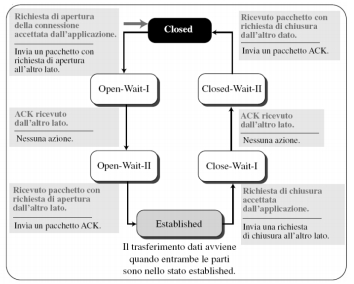
\includegraphics[width=.7\textwidth]{res/fsm.jpg} \hfill
\end{center}

\subsection{RDT 1.0}
Il caso riguardante \textit{RDT 1.0} è contestualizzato in una situazione perfettamente affidabile:
\begin{itemize}
    \item non si verificano \textbf{mai} errori nei bit trasmessi;
    \item non si verifica \textbf{mai} una perdita di pacchetti.
\end{itemize}
\begin{center}
    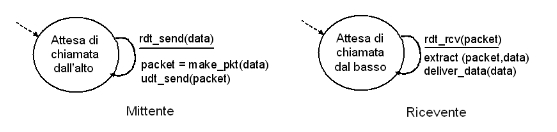
\includegraphics[width=.7\textwidth]{res/fsm-rdt-10.jpg} \hfill
\end{center}
\newpage

\subsection{RDT 2.0}
In questo caso, il canale di trasmissione effettiva può confondere i bit nel pacchetto. Da qui la necessità di introdurre dei messaggi di risposta alla ricezione di un pacchetto:
\begin{itemize}
    \item \textbf{ACK} (\textit{ACKnowledgment}, o \textit{conferma di ricezione}): utilizzato per confermare che il pacchetto è stato ricevuto ed è integro;
    \item \textbf{NAK} (\textit{Negative AcKnowledgment}, o \textit{conferma negativa}): il pacchetto contiene errori. Il mittente reinvia il pacchetto quando riceve indietro questo tipo di messaggio: motivo per cui si tratta di un protocollo \textit{ARQ} (\textit{Automatic Repeat reQuest}, o \textit{Richiesta Automatica di Ripetizione}.
\end{itemize}
\begin{center}
    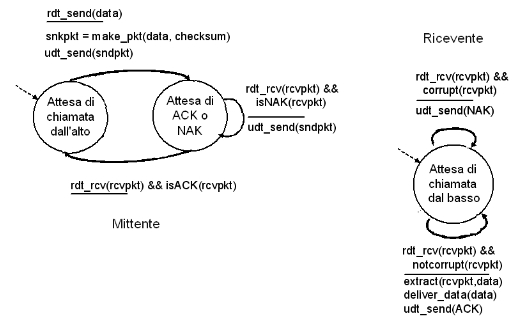
\includegraphics[width=.7\textwidth]{res/fsm-rdt-20.jpg} \hfill
\end{center}
\textit{RDT 2.0} può però andare incontro ad un difetto fatale: la mancata gestione degli eventi in cui i pacchetti \textit{ACK}/\textit{NAK} siano danneggiati.

\subsection{RDT 2.1}
Viene dunque aggiunto - alternativamente - un valore binario a ciascun pacchetto, un \textit{numero di sequenza}.
In questo modo, viene comunicato non solo l'esito della ricezione al mittente, ma anche il pacchetto a cui questo fa riferimento. \\
\begin{minipage}[t]{0.5\textwidth}
    \begin{center}
        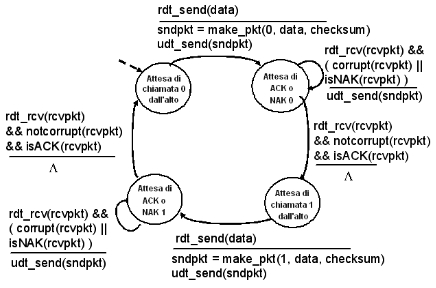
\includegraphics[width=.8\textwidth]{res/fsm-rdt-21-sender.jpg} \hfill
    \end{center}
\end{minipage}
\begin{minipage}[t]{0.5\textwidth}
    \begin{center}
        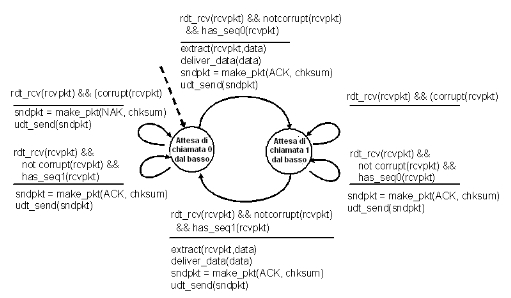
\includegraphics[width=.8\textwidth]{res/fsm-rdt-21-receiver.jpg} \hfill
    \end{center}
\end{minipage}
\newpage

\subsection{RDT 2.2}
\textit{RDT 2.2} fornisce le stesse funzionalità di \textit{RDT 2.1}, utilizzando però soltanto gli \textit{ACK}, escludendo i \textit{NAK}.
Nel caso in cui il destinatario dovesse inviare un \textit{NAK}, invia nuovamente un \textit{ACK} con numero di sequenza dell'ultimo pacchetto ricevuto correttamente.
\begin{center}
    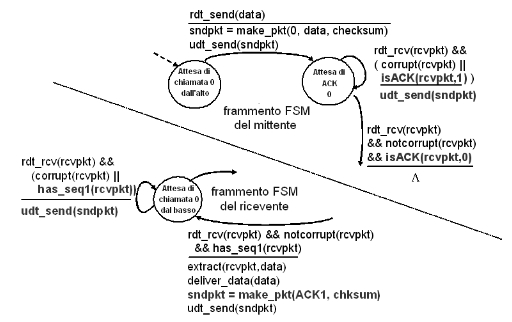
\includegraphics[width=.7\textwidth]{res/fsm-rdt-22.jpg} \hfill
\end{center}
L'alternativa è invece introdurre una nuova funzione di timing. Per ogni pacchetto inviato, il mittente implementa un timer: una volta che questo raggiunge un timeout, se non ha ricevuto nessun pacchetto che gli comunichi l'esito (l'\textit{ACK}), allora reinvia il pacchetto. Per questo motivo:
\begin{itemize}
    \item il mittente deve tenere una copia del pacchetto spedito fino a che non ne riceve riscontro dell'esito;
    \item per garantire il controllo di flusso, non si spedisce più di un pacchetto alla volta.
\end{itemize}